\chapter{Test}\label{Test}
I dette afsnit omtales test af PC Applikation. Som udgangspunkt er der lagt fokus på unit-tests. Der er kun lavet én integrationstest, som er en integrationstest af hele CalculationLibrary-projektets indhold. Det vil ikke være muligt at lave en integrationstest, hvor man bruger de lavestliggende moduler i hverken RoboLibrary eller ComputerVisionLibrary, da de hver især er afhængige af hardware. Klasserne der afhænger af hardware er derfor ikke unit-testet og er ekskluderet fra code coverage (CC). 
Efter unit-testen blev godkendt, er der kort tid efter, blevet udført system-test.

Da der ikke blev fundet nogen fornuftig måde at teste AutoSonographyWPF er den ej heller blevet testet, og er også udelukket fra CC.

\section{Test-specificering}
Hvert bibliotek i solutionen har et tilsvarende test-bibliotek. Hver testbar klasse i et bibliotek har en tilsvarende testklasse. Se figur \ref{SolutionStructure} for et overblik over testbibliotekerne. I tilfælde af at en klasse er afhængig af andre klasse, indsættes søm i form af interfaces. Dertil vil afhængighederne mockes ud i testene vha. dummy-klasser.

\begin{figure}[H]
    \centering
    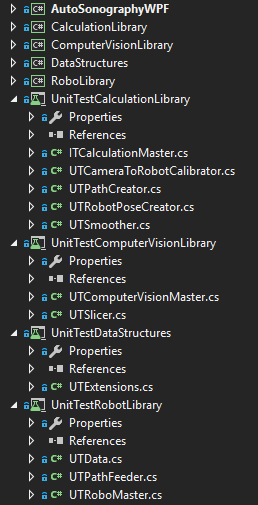
\includegraphics[width=0.3\textwidth]{figurer/d/Test/solution_overview}
    \caption{Solution struktur som set i Visual Studio's Solution Explorer}
    \label{SolutionStructure}
\end{figure}

\newpage
\subsection{Testklasse-opbygning}
Hver testklasse er erklæret med et 'TestClass' tag. Disse testklasser har en 'TestInitialize' metode der køres inden hver 'TestMethod' metode. I test-initialiseringen gennemkøres erklæringer der er fælles for alle test-metoderne. Hver test-metode er navngivet som 'MetodeDerTestes\_HvadDerGøres\_HvadDerForventes'. I test-metoderne bruges der 'Assert' for at verificere at de faktiske resultater der findes frem til stemmer overens med de forventede resultater. Her er et udpluk af unit-testen for klassen Slicer:

\begin{lstlisting}[language=Java]
...
namespace UnitTestRobotLibrary
{
	[TestClass]
	public class UTSlicer
	{
		private Slicer uut;
		private string testModelLocation;
		[TestInitialize]
		public void Setup()
		{
			uut = new Slicer();
			testModelLocation = Directory.GetParent(
				Directory.GetParent(
				Directory.GetParent(
				Environment.CurrentDirectory).
				ToString()).
				ToString()) +
				"\\TestModels";
		}

		[TestMethod]
		public void Slice_InsertFourFaces_2Returned()
		{
			string location = testModelLocation + @"\fourTriangles.ply";
			CVMesh mesh = PLYHandler.ReadMesh(location);
			float lowerLimit = 58.5f;
			float upperLimit = 1000f;
			Slicer.xMin = float.MinValue;
			Slicer.xMax = float.MaxValue;
			CVMesh sliced = uut.Slice(mesh, lowerLimit, upperLimit, false);
			Assert.AreEqual(5, sliced.Vertices.Count);
			Assert.AreEqual(0, sliced.Faces[0].index1);
			Assert.AreEqual(1, sliced.Faces[0].index2);
			Assert.AreEqual(2, sliced.Faces[0].index3);
			Assert.AreEqual(3, sliced.Faces[1].index1);
			Assert.AreEqual(2, sliced.Faces[1].index2);
			Assert.AreEqual(4, sliced.Faces[1].index3);
		}
		...
	}
}
\end{lstlisting}
I metoden 'Setup' erklæres stien for mappen hvor de modeller som unit-testen skal teste på ligger, og unit under test (uut) oprettes på ny. Der tjekkes med Assert om resultaterne er korrekte. Såfremt at en af 'AreEqual'-metoderne returnerer 'false', vil testen fejle.
\newpage
\section{Resultater}
Der blev skrevet 42 tests som alle gik igennem pr d. 7/12/2016.
Se bilag \ref{TestResultater} Testresultater for en oversigt over disse tests og deres resultater.

Disse 42 tests resulterede i en code coverage på 96\%. Se figur \ref{CodeCoverage} for overblik, og se bilag \ref{Code Coverage} Code Coverage for en interaktiv navigering af code coveragen. 

\begin{figure}[H]
    \centering
    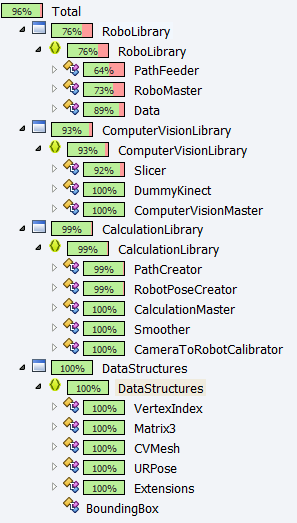
\includegraphics[width=0.3\textwidth]{figurer/d/Test/coverage}
    \caption{Code coverage udregnet af ReSharper-værktøjet}
    \label{CodeCoverage}
\end{figure}

Code coveragen siger noget om hvor stor en procentdel af den kode, der er valgt at blive inkluderet, som er blevet gennemløbet af unit-tests. Det vil sige at nogle klasser er blevet eksluderet fra denne coverage. Disse elementer fra kravspecifikationen er ikke blevet 'coveret' eller testet:
\begin{itemize}
\setlength\itemsep{0.25em}
\item{\textbf{AutosonographyWPF}} - Kræver simulering af musetryk m.m.
\item{\textbf{ComputerVisionLibrary:KinectFusionizer}} - Kræver tilslutning af hardware
\item{\textbf{RoboLibrary:Analyzer}} - Kræver tilslutning af hardware
\item{\textbf{RoboLibrary:ModBus}} - Kræver tilslutning af hardware
\item{\textbf{RoboLibrary:Reader}} - Kræver tilslutning af hardware
\item{\textbf{RoboLibrary:Writer}} - Kræver tilslutning af hardware
\end{itemize}

Derudover er der også ekskluderet diverse metoder og få klasser der kun har til formål at debugge PC Applikation.